\section{权重结构的补充分析}
\label{sec:sup:weight-structure}

\subsection{网格与分类}
正文图~\ref{fig:joint:phase}在 $r\in[0.9,20]$ 的 $300$ 个对数等距点与 $S\in(S_c,S^*]$ 的 $300$ 个等距点上逐状态求解，正文讨论其中 $r\ge1$ 的部分，跳变位置在 $S$ 上二分定位；默认的 $r=2$ 由正文第~\ref{sec:joint:compare-numerics}~节单独计算。表~\ref{tab:joint:weight-transitions}给出成本最优控制的结构转折所在的 $r$ 括区。括区由 $r\in[0.1,20]$ 内 $161$ 个对数等距点的原网格出发确定：对全部网格点重新分类，在类别不同的相邻网格点之间取 $20$ 个细分点，找出每个改变区间，再在 $\log r$ 上二分到宽度小于 $10^{-3}$，不假定结构类别对 $r$ 单调；各括区在 $N_z=8001$ 与 $16001$ 下类别不变。结构 A$'$ 中的内部跳变另用不依赖根法的 $2\times10^{5}$ 点网格逐点核对：两个内部局部极小在跳变处交换全局最优，两个分支的成本相对只差约 $10^{-5}$。

\subsection{结构边界}
表~\ref{tab:joint:weight-transitions}的前两个转折可以与闭式比较。正文定理~\ref{thm:joint:cost-structure}的权重界 $r_{\rm cont}$（式\eqref{eq:joint:rcont}）保证控制连续，两组参数下的值都落在 A$\to$A$'$ 的括区内；A$'\to$B 的转折由下面的命题给出。
\begin{proposition}
\label{prop:sup:rhat}
设 $w_c,w_q>0$，$r=w_q/w_c$，不考虑能力约束。对一切 $S>S_{\rm sw}$，$c=c_0$ 都是 $f(S,\cdot)$ 在 $[c_0S_c/S,c_0]$ 上的唯一全局最小点，当且仅当
\[
r\le\hat r=\Bigl(\frac{S_{\rm sw}}{S_{\rm sw}-S_c}\Bigr)^2 .
\]
此外 $9/4<\hat r<4$，且 $r_{\rm cont}<\hat r$。
\end{proposition}
\begin{proof}
沿用正文附录~\ref{sec:proof:cost-structure}的记号 $\zeta,p,G=A+rB$。先证上集性：若 $p=\zeta_0$ 是 $G(\cdot;\zeta_0)$ 的全局最小点，则对任意 $\zeta_1>\zeta_0$，$p=\zeta_1$ 是 $G(\cdot;\zeta_1)$ 的唯一全局最小点。由正文命题~\ref{prop:joint:global-structure}，$\zeta_0\ge\zeta_{\rm sw}$。对固定 $p<\zeta$，$A$ 关于 $\zeta$ 严格增；$B$ 与 $\zeta$ 无关，且 $B'(p)=-(p-1)(p^2-3p+2b)/[p^3(p-b)^2]$，故 $B$ 在 $[\zeta_{\rm sw},\infty)$ 上严格减。$p\le\zeta_0$ 时，$G(p;\zeta_1)>G(p;\zeta_0)\ge rB(\zeta_0)\ge rB(\zeta_1)=G(\zeta_1;\zeta_1)$；$\zeta_0<p<\zeta_1$ 时，$G(p;\zeta_1)\ge rB(p)>rB(\zeta_1)$。

再看 $S_{\rm sw}$ 处。令 $x=c/c_0\in[\sigma,1]$，$\sigma=S_c/S$，$a=(1-\sigma)^2$，$d=1-b\sigma$。利用恒等式 $d(x-\sigma)^2-ax^2(x-b\sigma)=(1-x)P(x)$，$P(x)=ax^2-d\sigma(2-\sigma)x+d\sigma^2$，对 $x\in[\sigma,1)$，$f(S,c_0x)\ge f(S,c_0)$ 等价于 $d(1-x)x^2+rP(x)\ge0$。在 $\sigma=S_c/S_{\rm sw}$ 上 $2b\sigma^2-3\sigma+1=0$，即 $2\sigma d=1-\sigma$，于是 $P(x)=a(x-1)(x-x_2)$，$x_2=\sigma/[2(1-\sigma)]<\sigma$。条件化为：对一切 $x\in[\sigma,1)$ 有 $r(x-x_2)\le(d/a)x^2$。比值 $(d/a)x^2/(x-x_2)$ 在 $x=2x_2=\sigma/(1-\sigma)\in(\sigma,1)$ 取最小值 $4x_2d/a=1/(1-\sigma)^2=\hat r$。

若 $r<\hat r$，$c_0$ 是 $S_{\rm sw}$ 处的唯一全局最小点；若 $r=\hat r$，它与 $x=2x_2$ 并列。两种情形下，由上集性，对一切 $S>S_{\rm sw}$，$c_0$ 都是唯一全局最小点。若 $r>\hat r$，则在 $S_{\rm sw}$ 处存在 $x<1$ 使 $f(S,c_0x)<f(S,c_0)$；由连续性，这一严格不等式在 $S_{\rm sw}$ 稍上方仍成立。最后，$S_{\rm sw}/S_c\in(2,3)$ 给出 $9/4<\hat r<4$；由 $\zeta_{\rm sw}=S_{\rm sw}/S_c$ 得 $b=\zeta_{\rm sw}(3-\zeta_{\rm sw})/2$，不等式 $r_{\rm cont}<\hat r$ 化为 $(\zeta_{\rm sw}-1)(\zeta_{\rm sw}-2)^2>0$。
\end{proof}
$\hat r$ 的含义是：隔离的相对权重超过它以后，在 $S_{\rm sw}$ 稍上方同时减少接触已经更省；若存在仅隔离段，它就会在到达 $S_{\rm sw}$ 前结束。
\begin{table}[htbp]
\centering\small
\renewcommand{\arraystretch}{1.2}
\begin{threeparttable}
\caption{权重网格上成本最优控制的结构转折}
\label{tab:joint:weight-transitions}
\begin{tabular*}{\linewidth}{@{\extracolsep{\fill}}llcccc@{}}
\toprule
 & & \multicolumn{2}{c}{基准} & \multicolumn{2}{c}{西安}\\
\cmidrule(lr){3-4}\cmidrule(l){5-6}
转折 & 结构变化 & 闭式 & 括区 & 闭式 & 括区\\
\midrule
A$\to$A$'$ & 出现内部跳变 & $r_{\rm cont}=\nrCostRcontBase$ & $[\nrWtBaseAToApLo,\nrWtBaseAToApHi]$ & $r_{\rm cont}=\nrCostRcontXian$ & $[\nrWtXianAToApLo,\nrWtXianAToApHi]$\\
A$'\to$B & 切换提前并跳变 & $\hat r=\nrCostRhatBase$ & $[\nrWtBaseApToBLo,\nrWtBaseApToBHi]$ & $\hat r=\nrCostRhatXian$ & $[\nrWtXianApToBLo,\nrWtXianApToBHi]$\\
B$\to$C & 仅隔离段消失 & — & $[\nrWtBaseBToCLo,\nrWtBaseBToCHi]$ & — & $[\nrWtXianBToCLo,\nrWtXianBToCHi]$\\
\bottomrule
\end{tabular*}
\begin{tablenotes}[flushleft]\footnotesize
\item 注：$w_c=1$，$r=w_q/w_c$，不考虑能力约束。结构 A：在 $S_{\rm sw}$ 处连续切换，此后控制连续；A$'$：在 $S_{\rm sw}$ 处连续切换，随后在 $S_{\rm sw}$ 稍下方于两个内部取值之间跳变一次；B：切换提前到 $S_{\rm sw}$ 以上，接触率在切换处跳变；C：没有仅隔离段。括区是所检验网格与精度下含该转折的 $r$ 括区，宽度小于 $10^{-3}$；闭式列中 $r_{\rm cont}$ 为正文定理~\ref{thm:joint:cost-structure}的连续界（充分条件），$\hat r$ 见命题~\ref{prop:sup:rhat}。
\end{tablenotes}
\end{threeparttable}
\end{table}

图~\ref{fig:sup:phase-detail}放大正文图~\ref{fig:joint:phase}的转折区。数值上，内部跳变从 $r=r_{\rm cont}$ 处开始（空心圆），连续切换与由仅隔离控制出发的跳变在 $(S_{\rm sw},\hat r)$ 处相接（空心菱形）。
\begin{figure}[htbp]
\centering
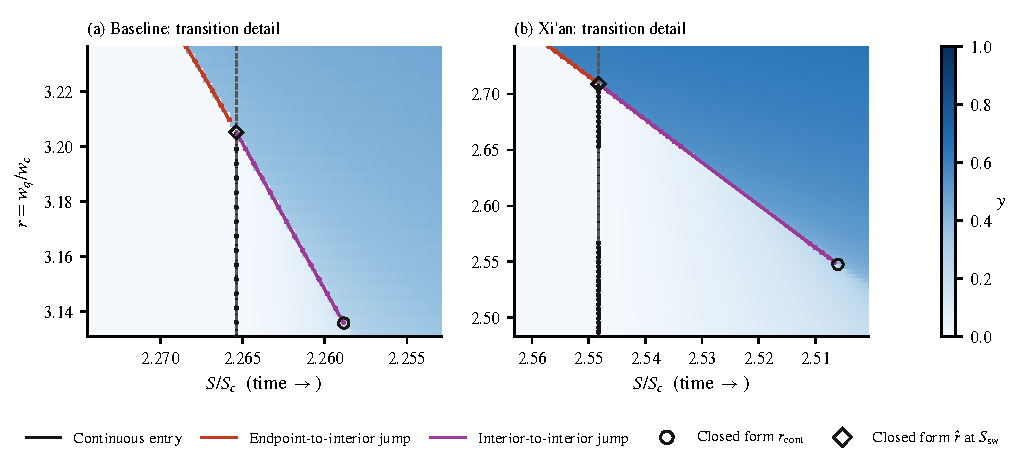
\includegraphics[width=\textwidth]{figures/joint_v2/joint_phase_detail.pdf}
\caption{正文图~\ref{fig:joint:phase}转折区的局部加密。(a) 基准参数；(b) 西安参数。颜色为 $y$；点为表~\ref{tab:joint:weight-transitions}所涉加密权重及西安两处补充计算点上的局部分类，黑线为连续进入内部分支的边界，红线为端点到内部的跳变，紫线为两个内部取值之间的跳变。空心圆位于 $r=r_{\rm cont}$（正文式\eqref{eq:joint:rcont}）、$S/S_c=b+\sqrt{b^2-8b+8}$，空心菱形为 $(S_{\rm sw}/S_c,\hat r)$（命题~\ref{prop:sup:rhat}）。随时间推进，$S$ 从左向右减小。}
\label{fig:sup:phase-detail}
\end{figure}
\FloatBarrier
